% ##CHRIS 2026-09-22: Paper 1 draft v1, complete. IEEEtran journal, two columns.
% Every number carries a % TODO-source line naming the file in ../experiments/final it came from.
% Nothing is quoted that is not in a file. Figures that do not exist yet are listed at the end of
% this source under "FIGURES NOT YET MADE" rather than invented.
\documentclass[journal]{IEEEtran}
\usepackage{amsmath,amssymb,booktabs,graphicx,microtype}
\usepackage[dvipsnames]{xcolor}
\usepackage[colorlinks=true,linkcolor=NavyBlue,urlcolor=NavyBlue,citecolor=NavyBlue]{hyperref}
\newcommand{\kT}{k_{\mathrm B}T}
\newcommand{\avg}[1]{\left\langle #1 \right\rangle}
\newcommand{\dd}{\mathrm{d}}
\graphicspath{{../experiments/final/}}

\begin{document}

\title{The speed of sound in a two-dimensional hard-disk gas:\\
a divider-mode measurement against the equation of state}

\author{Christoph~Haring and Susanne~Still%
\thanks{The authors are with the Department of Information and Computer Sciences,
University of Hawai\`i at M\=anoa, Honolulu, HI 96822 USA
(e-mail: charing@hawaii.edu; sstill@hawaii.edu).}}

\maketitle

\begin{abstract}
% TODO-source: 260919_A1v2_final_cs_vs_eta.csv (35 densities, 7873 health-clean trajectories)
We measure the adiabatic speed of sound of a hard-disk fluid from the eigenfrequency of a massive
divider separating two compartments, the method of Rom\'an \emph{et al.}, over 35 packing fractions
from $\eta = 0.0065$ to $0.76$ and nine divider masses per density. The measurement is compared with
the Kolafa--Rottner equation of state through the adiabatic relation
$c_s^2 = (\kT/m)[Z + \eta Z' + Z^2]$ with no fitted parameter. For $\eta \le 0.4$ the agreement is
$+1.04\,\%$ on average at $N = 100$; a size ladder to $N = 2500$ shows the offset is finite size. We
bound the estimator's own systematic below $0.3\,\%$, and we show that the apparent
density-dependent excess reported in 2002 is an artefact of the $\gamma = 2$ mapping used then:
re-mapped adiabatically, that 24-year-old data set shows the same flat $+1.1\,\%$ offset as ours,
in the same box.
\end{abstract}

\begin{IEEEkeywords}
hard-disk fluid, speed of sound, event-driven molecular dynamics, equation of state,
finite-size scaling
\end{IEEEkeywords}

\section{Introduction}
\IEEEPARstart{T}{he} hard-disk fluid is the simplest system with a non-trivial equation of state,
and its thermodynamics is known to high precision from simulation~\cite{kolafa2006}. Its
\emph{dynamical} response is measured less often. The speed of sound is the natural bridge: for a
two-dimensional monatomic fluid it is fixed entirely by the equation of state,
\begin{equation}
c_s^2 = \frac{\kT}{m}\left[Z + \eta Z' + Z^2\right],
\label{eq:adiabatic}
\end{equation}
so a measurement of $c_s$ tests $Z(\eta)$ with the equation of state as an \emph{input} rather than
a fit. Agreement is then a check; disagreement is a measurement of something the equation of state
does not contain.

Measuring $c_s$ by launching a pulse needs a large box and care with the pulse amplitude. Rom\'an
\emph{et al.}~\cite{roman2002} avoid both by placing a massive divider between two compartments and
watching it ring: the divider is a mass on two gas springs and its eigenfrequency is set by $c_s$.
The measurement becomes a frequency, which is cheap to make precise, and the system can be small.
We adopt that apparatus, and much of this paper is about what it takes to trust the frequency it
returns.

Two things motivate revisiting it. First, the estimator. The divider carries a second, much slower
motion that is not the sound mode, whose spectral weight can exceed the resonance; an unguarded
peak-finder is wrong by tens of per cent (\S\ref{sec:estimator}). Second, the comparison. Rom\'an
\emph{et al.} convert $Z$ to $c_s$ with a constant $\gamma = 2$ and report an excess over theory
that grows with density; we show in \S\ref{sec:roman} that the growth is the mapping, and that their
data and ours then agree.

\section{Model and apparatus}\label{sec:apparatus}
Hard disks of diameter $\sigma = 2r$ and mass $m$ occupy a box of height $H$ split at the centre by
a divider of mass $M$ and thickness $t$, with $N_s$ disks on each side. Units are reduced,
$\kT = m = \sigma = 1$; we use $H = 10$ and $N_s = 50$ unless stated.
% TODO-source: geometry constants in hspist3/validation/tests_20260913.py (N_TOTAL, N_SIDE, RDISK, H, WALL_T)

\begin{figure}[t]\centering
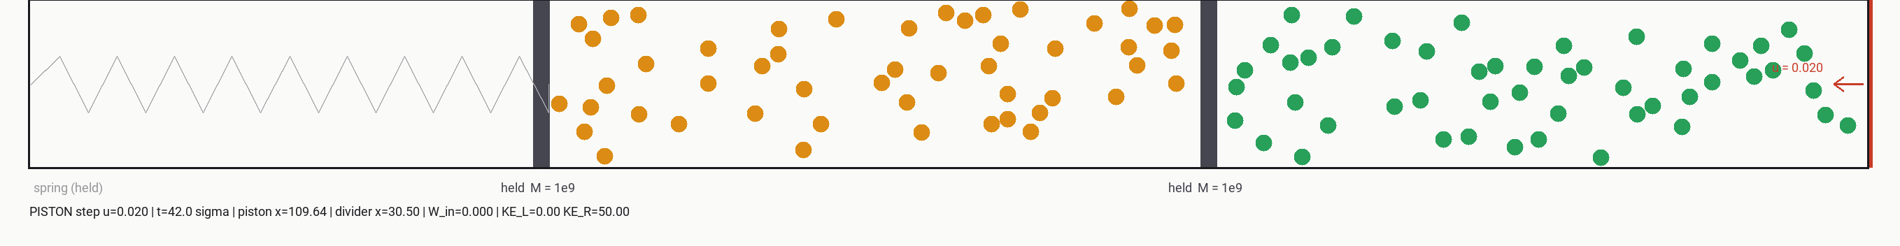
\includegraphics[width=\linewidth]{260922_apparatus_paper.png}
\caption{The apparatus, drawn by the simulation itself. Two compartments of 50 disks either side of
the divider. Walls are labelled by mass; a held wall is drawn solid and a free one hollow. The wall
at left bounds an inert compartment belonging to a companion experiment and is held immovable
throughout this work.}
\label{fig:apparatus}
\end{figure}

The dynamics are event-driven and exact between collisions; all results use the scientific backend.
The divider is held for an equilibration period, during which each compartment is separately
equalised to $KE = N_s\kT$, and is then released; its position $x(t)$ is recorded at fixed sampling
interval. Every trajectory is checked against a health contract --- a scheduler forced advance, an
overlap repair, a wall-position clamp or an overdue wall collision each discard that trajectory,
never the cell. Of 7875 trajectories in the main campaign, 2 were discarded.
% TODO-source: 260913_tests_STATUS.md, A1 v2 campaign close-out

\paragraph{Effective length} The disk centres in one compartment span $r$ to $L_0 - t/2 - r$, so the
length entering the mode is
\begin{equation}
L_{\mathrm{eff}} = L_0 - 2r - t/2 .
\label{eq:leff}
\end{equation}
Carrying $t$ lowers every $c_s$ by $(t/2)/(L_0-2r)$: $0.004\,\%$ at $\eta = 0.0065$ and $0.50\,\%$
at $\eta = 0.65$. The density is defined on the physical area, $\eta = N_s\pi r^2/(L_0H)$, with no
exclusion --- $L_{\mathrm{eff}}$ is an acoustic length and enters nowhere else.
% TODO-source: validation/paper1_canonical_20260919.py; 260919_A1v2_final_cs_vs_eta.csv

\section{The estimator}\label{sec:estimator}
For each trajectory we form the periodogram of the divider position,
\begin{equation}
P(f) = \Big|\sum_j \big(x(t_j) - \bar x\big)\,e^{-2\pi i f t_j}\Big|^2 ,
\end{equation}
and take the largest bin at or above a one-sided floor,
\begin{equation}
\nu = \arg\max_{f \,\ge\, \nu_{\mathrm{pred}}/X} P(f), \qquad X = 2.5 ,
\label{eq:estimator}
\end{equation}
then average over 25 seeds. With record length $T$ the bin width is $1/T$, so at 200 predicted
periods the rounding floor on one frequency is $100/(N_{\mathrm{cyc}}\sqrt{12}) = 0.144\,\%$.
% TODO-source: 260913_method_roman_fft_COWORK.md section 1

\paragraph{Why a floor is needed} Besides the resonance the divider performs a slow wander: a
five-period running mean of $x$ carries $9$--$57\,\%$ of the variance of $x$. It is not a start-up
transient --- its variance is the same in the second half of a record as the first, and a
hundredfold longer hold does not change it --- and it is a relaxation rather than an oscillation,
with a correlation time of 53--102 acoustic periods. It is the adiabatic-piston mechanism: thermal
fluctuations of the two compartment temperatures shift the pressure balance, the divider follows,
and it returns only as heat crosses the divider. A dedicated run logging the compartment kinetic
energies confirms it directly, with correlation $r = +0.978$ between the slow mode and the
temperature difference and the amplitude reproduced to $6$--$7\,\%$ by
$x = (L_0/2)(\Delta T/T)\,Z/(Z+\eta Z')$. Its power sits at low frequency, and at $\eta \ge 0.52$ it
reaches $85$--$280\,\%$ of the resonance peak for the lightest divider.
% TODO-source: 260913_method_roman_fft_COWORK.md section 7; adiabatic_piston_check_20260913/step3_results.json

The consequence is quantitative. Against a reference that windows the spectrum around the
resonance, an unguarded largest bin is wrong by up to $33\,\%$ on 25-period records and \emph{up to
$93\,\%$ at 200 periods} --- the error grows with record length, because a longer record resolves
the wander into more bins, any of which can outgrow the resonance. Short records hide the problem
rather than remove it. The floor removes it, and the answer does not depend on where the floor is
placed: every $X$ from $2.08$ to $6.25$ gives the identical $c_s$ at 200 periods.
% TODO-source: 260914_A1v2_kmin_sensitivity.csv, 260914_A1v2_kmin_sensitivity_extended.csv

\paragraph{Largest bin or a fit?} A resonance fit to each trajectory is the obvious alternative and
the more precise one. Both put the nine masses of \S\ref{sec:ladder} on a single line to
$0.27\,\%$. But a biased estimator does not scatter about the line, it leans: regressing the
residual on $\ln\alpha$ gives $-0.286 \pm 0.020\,\%$ per e-fold for the fit ($14.4\sigma$) against
$-0.030 \pm 0.029\,\%$ for the largest bin ($1.0\sigma$, flat). The fit walks monotonically from
$+0.35\,\%$ at the lightest divider to $-0.64\,\%$ at the heaviest. We use the largest bin and
report the fit as a cross-check; no equation of state entered that choice.
% TODO-source: 260913_method_roman_fft_COWORK.md section 3.1; validation/estimator_massladder_20260917.py

\paragraph{Bounding the rest} Damping shifts the position-spectrum peak below the eigenfrequency by
$\Gamma^2/4f_0^2$; with the measured $\Gamma/f_0 = 0.023$ (median, $\eta<0.5$) and $0.063$
($\eta\ge0.5$) that is at most $0.34\,\%$, typically $0.01$--$0.11\,\%$. Weighting by $(2\pi f)^2$
to suppress the slow mode without a floor was tested and rejected: it moves $c_s$ by $+0.02$ to
$+3.3\,\%$, one-signed and largest at high density, which is a spectral-shape systematic and not
noise. Taken together the estimator's own systematic is below $0.3\,\%$, against the $1$--$3\,\%$
effects the paper reports.
% TODO-source: 260915_A1v2_damping_test.csv; 260914_A1v2_velocity_spectrum_test.csv


\begin{figure}[t]\centering
\includegraphics[width=\linewidth]{261001_p1_slowmode.pdf}
\caption{Why the floor exists. \textbf{Left:} the divider displacement at $M = 1000$,
$\eta = 0.1122$, with its five-period running mean --- the slow adiabatic-piston wander, which
carries no information about $c_s$ but has more low-frequency power than the resonance.
\textbf{Right:} the same record's periodogram. Without a floor the largest bin is the wander, not
the mode; the estimator therefore takes the largest bin at $f \geq \nu_{\rm pred}/2.5$.}
\label{fig:slowmode}
\end{figure}

\begin{figure}[t]\centering
\includegraphics[width=\linewidth]{261001_p1_estimator_floor.pdf}
\caption{Floor sensitivity. Median $|\Delta c_s|$ against the windowed reference over all 35
densities, with the $16$--$84\,\%$ spread as the error bar, versus the floor parameter $X$ (the
floor is $\nu_{\rm pred}/X$, so a \emph{large} $X$ is a \emph{low} floor). The collapse at large
$X$ is the slow mode of Fig.~\ref{fig:slowmode} winning the periodogram; it is worse at 200
periods, where the wander has more bins below the resonance. At the production value $X = 2.5$ the
estimator reproduces the windowed reference exactly at both record lengths.}
\label{fig:floor}
\end{figure}

\section{The mass ladder}\label{sec:ladder}
Linearising about the symmetric position makes the divider a mass on two gas springs. Writing the
displacement field in each compartment as a standing wave of wavenumber $k$, imposing continuity at
the divider faces and Newton's law for the divider,
$M\ddot\xi = -[p_{\mathrm{right}} - p_{\mathrm{left}}]H$, gives with $K = kL$
\begin{equation}
\cot K = \alpha K , \qquad \alpha = \frac{M}{2N_s m} ,
\label{eq:transcendental}
\end{equation}
whose lowest root fixes the fundamental,
\begin{equation}
\nu = \frac{c_s K(\alpha)}{2\pi L_{\mathrm{eff}}} .
\label{eq:nu}
\end{equation}
Two limits are worth recording. For a heavy divider $K^2 \to 2N_s m/M$, so the divider becomes a
mass on a spring of stiffness $N_s m c_s^2/L^2$ per compartment --- the gas spring is the sound
speed. For a light divider $K \to n\pi/2$ with $n$ odd; the even standing modes are absent because
they have a node where the divider sits.

Equation~\eqref{eq:nu} is linear in $K(\alpha)$ through the origin, which makes the mass ladder a
self-contained consistency test: a single $c_s$ must place every mass on the same line, with no
equation of state involved. We use nine masses, $M = 50$ to $2000$, and take $c_s$ as the
through-origin slope of $\bar\nu_M$ against $K(\alpha)/2\pi L_{\mathrm{eff}}$, its uncertainty being
the scatter of the per-mass values about that line. That scatter, $0.27\,\%$, is within a factor two
of the bin-rounding floor.
% TODO-source: 260919_A1v2_final_cs_vs_eta.csv columns c_s, c_s_scatter_mass, n_masses


\begin{figure}[t]\centering
\includegraphics[width=\linewidth]{261001_p1_massladder_line.pdf}
\caption{One worked mass ladder, $\eta = 0.1122$, nine divider masses $M = 50$--$2000$, 25 seeds
each. \textbf{Left:} $\bar\nu_M$ against $x_M = K(\alpha)/2\pi L_{\rm eff}$ with $K$ the root of
$\cot K = \alpha K$; the slope through the origin is $c_s$. \textbf{Right:} residuals about that
line, flat across a factor 40 in $M$. The measured $c_s$ sits $1.0\,\%$ above Kolafa--Rottner, the
finite-size offset discussed in \S\ref{sec:finitesize}.}
\label{fig:ladderline}
\end{figure}

\begin{figure}[t]\centering
\includegraphics[width=\linewidth]{261001_p1_massladder_residuals.pdf}
\caption{Mass independence, the ladder's one assumption, tested. Mean residual about each density's
own ladder line at fixed $\alpha = M/2N_sm$, averaged over the 24 densities with $\eta \leq 0.69$,
against $\ln\alpha$. The largest-bin estimator is flat; the per-trajectory fit drifts by an order
of magnitude more per e-fold in $\alpha$, which is why the largest bin is the production
estimator.}
\label{fig:ladderres}
\end{figure}

\section{Results}\label{sec:results}
\begin{figure*}[t]\centering

\includegraphics[width=0.86\textwidth]{260919_cs_vs_eta.pdf}
\caption{$c_s(\eta)$ at $N = 100$ against three equations of state, through \eqref{eq:adiabatic}
with no fitted parameter. Shading marks the regimes, with the transition densities taken from
Engel \emph{et al.}~\cite{engel2013}: liquid--hexatic coexistence over
$0.700 \lesssim \eta \lesssim 0.716$ and the hexatic--solid crossover near $\eta = 0.720$. Points
beyond $\eta \approx 0.69$ lie in that region, where no fluid reference exists; they are shown but
are not counted as a deviation from Kolafa--Rottner.}
\label{fig:csvseta}
\end{figure*}

% TODO-source: 260919_A1v2_final_cs_vs_eta.csv, column dev_KR_pct
Over $\eta \le 0.4$ the measurement sits $+1.04\,\%$ above Kolafa--Rottner on average at $N = 100$
and never worse than $1.68\,\%$. The offset is one-signed and grows slowly with density.

\begin{figure}[t]\centering

\includegraphics[width=\linewidth]{260919_cs_vs_eta_lowdensity_zoom.pdf}
\caption{The dilute end. The $N = 100$ curve sits $0.5$--$1.5\,\%$ above the equation of state;
larger systems agree with it within their errors.}
\label{fig:zoom}
\end{figure}

\section{Finite size}\label{sec:finitesize}
% TODO-source: 260917_A2_cs_vs_N_extrapolation.csv, 260916_A2_finite_size_forms.csv
Along $N = 100, 400, 900, 1600$ (and 2500 where available) at fixed $\eta$, $c_s(N)$ is fitted with
$c_\infty + b/\sqrt N$, with $b/N$ and the two-term form bracketing the systematic. At
$\eta = 0.02$, $c_\infty = 1.4614 \pm 0.0102$ against $1.4725$ from the equation of state
($-1.1\sigma$); at $\eta = 0.05$, $1.5699 \pm 0.0029$ against $1.5666$ ($+1.1\sigma$). The $N = 100$
offset closes as the box grows: it is finite size, not a defect of the method.

\begin{figure}[t]\centering

\includegraphics[width=\linewidth]{260919_cs_vs_eta_N100_vs_A2.pdf}
\caption{$N = 100$ against $N = 900$ and $1600$ at the same densities.}
\label{fig:n100}
\end{figure}

\paragraph{What the offset is not} The pressure measured at the wall of the same finite box exceeds
the bulk equation of state by $7$--$20\,\%$, rising with $\eta$. Propagated through
\eqref{eq:adiabatic} that would imply a $+5$ to $+16\,\%$ excess in $c_s$, five times what is
observed. The pressure of a finite box and its sound speed are therefore two \emph{different}
finite-size quantities, and the bulk relation between them does not hold at $N = 100$. We report
this as a negative result: the wall pressure cannot be used to explain the offset.
% TODO-source: appendix C2 of 260919_paper2_ramp_linewidth_fast_REPORT.md, 120 hold runs

\section{Comparison with Rom\'an \emph{et al.} (2002)}\label{sec:roman}
% TODO-source: 260922_roman2002_remapped_vs_KR.csv; validation/roman2002_remapped_20260922.py
Rom\'an \emph{et al.}~\cite{roman2002} measured the same observable in the same box ($N_s = 50$,
$H = 10$) and report $c_s$ above scaled-particle theory and Henderson by an amount that \emph{grows}
with density, from $+1.3\,\%$ at $\eta = 0.112$ to $+12.8\,\%$ at $0.524$. That growth is the
mapping. They convert $Z$ to $c_s$ with a constant $\gamma = 2$; using \eqref{eq:adiabatic} on their
own numbers gives Table~\ref{tab:roman}.

\begin{table}[t]
\centering
\caption{Rom\'an \emph{et al.} Table I re-mapped. $\eta$ is recomputed from their $L_0$.}
\label{tab:roman}
\small
\begin{tabular}{@{}lcccc@{}}
\toprule
$L_0$ & $\eta$ & $c_s$ (theirs) & dev., $\gamma=2$ & dev., adiabatic \\
\midrule
7.5  & 0.5236 & $5.99 \pm 0.09$ & $+10.6\,\%$ & $+1.0\,\%$ \\
10   & 0.3927 & $3.78 \pm 0.08$ & $+5.5\,\%$  & $+0.9\,\%$ \\
15   & 0.2618 & $2.61 \pm 0.03$ & $+3.3\,\%$  & $+1.5\,\%$ \\
20   & 0.1963 & $2.20 \pm 0.02$ & $+1.9\,\%$  & $+0.9\,\%$ \\
25   & 0.1571 & $2.01 \pm 0.02$ & $+1.9\,\%$  & $+1.3\,\%$ \\
30   & 0.1309 & $1.89 \pm 0.02$ & $+1.5\,\%$  & $+1.1\,\%$ \\
35   & 0.1122 & $1.81 \pm 0.02$ & $+1.3\,\%$  & $+1.0\,\%$ \\
\bottomrule
\end{tabular}
\end{table}

The density-dependent excess becomes a flat $+1.10\,\%$ (spread $+0.91$ to $+1.46\,\%$), against our
$+1.04\,\%$ at $N = 100$ averaged over $\eta \le 0.4$. Two independent implementations, 24 years
apart, in the same box, with the same offset: that makes the $+1\,\%$ a property of the $N = 100$
divider apparatus rather than of either code. Their own size series (their Table II,
$N = 64 \to 4096$, $c_s = 3.81 \to 3.75$, extrapolating to $3.74$) runs in the same direction as
ours. As a transcription check, their scaled-particle and Henderson columns are reproduced to every
printed digit by our equation-of-state code together with their $\gamma = 2$ mapping.

The two measurements differ at one point, $\eta \approx 0.52$: ours sits $+2.6\,\%$ and theirs
$+1.0 \pm 1.5\,\%$, which is $1.1\sigma$ on their error bar alone, with 100 trajectories against our
25.

\begin{figure}[t]\centering
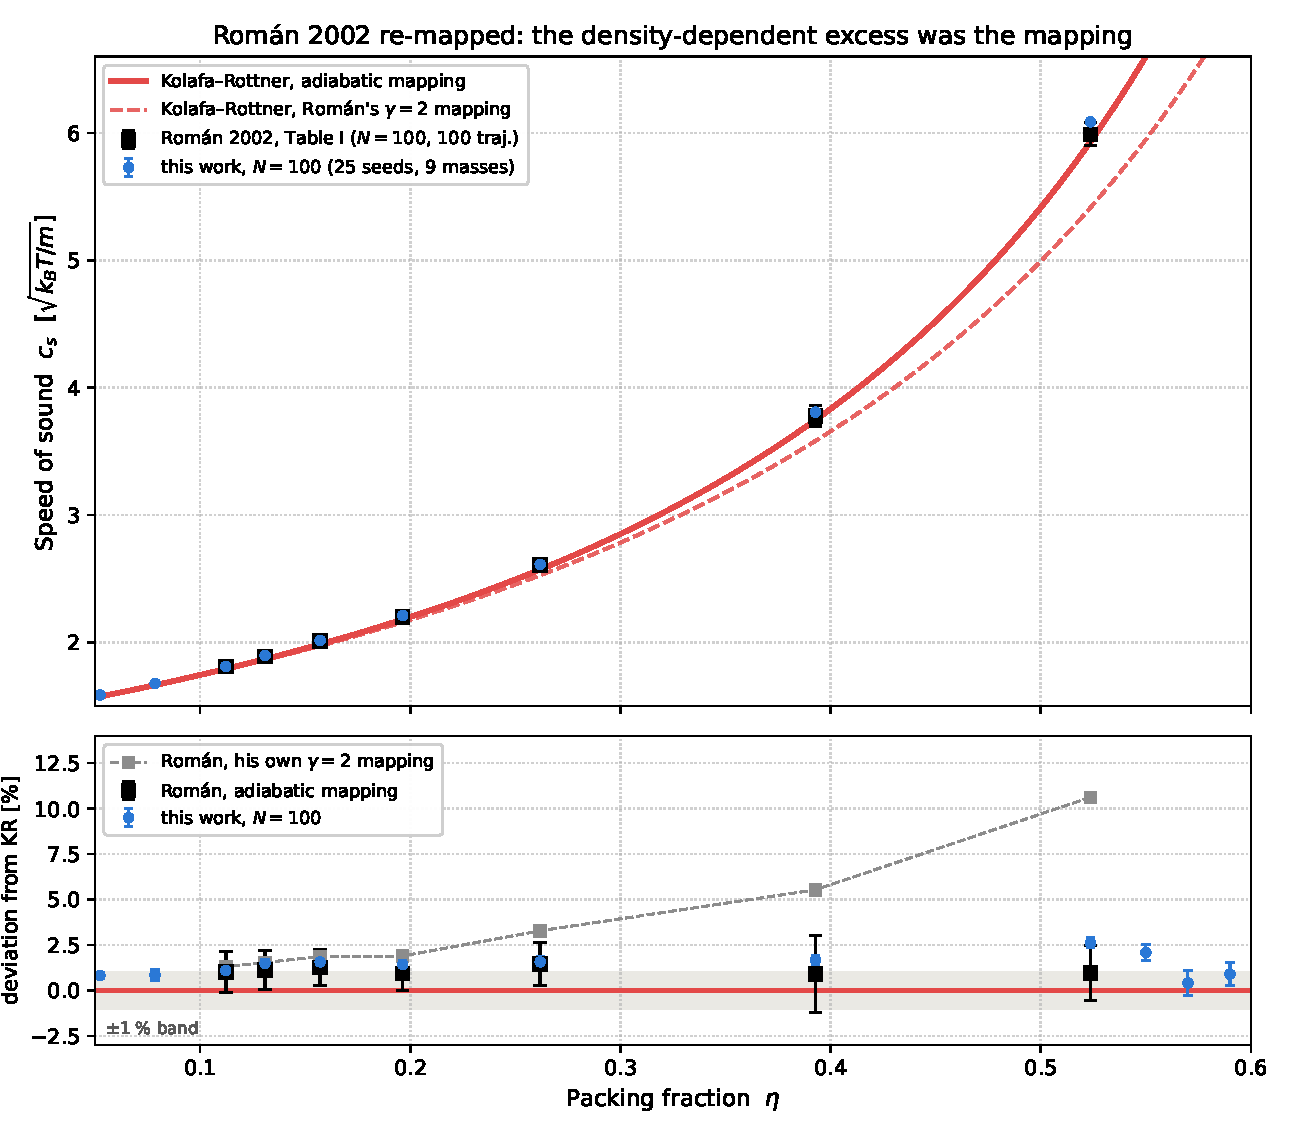
\includegraphics[width=\linewidth]{260922_roman2002_remapped_vs_KR.pdf}
\caption{Rom\'an \emph{et al.} re-mapped. Solid red, Kolafa--Rottner through \eqref{eq:adiabatic};
dashed red, the same equation of state through their $\gamma = 2$ mapping; black squares, their
Table I with their error bars; blue, this work at $N = 100$. Lower panel: deviation from
Kolafa--Rottner.}
\label{fig:roman}
\end{figure}

\subsection{Above $\eta \approx 0.69$: the right comparison is not Kolafa--Rottner}
\label{sec:ordering}
Kolafa--Rottner is a \emph{fluid} equation of state fitted below the transition, so a deviation
from it above $\eta \approx 0.69$ measures the extrapolation, not the gas. The reference there is
Engel \emph{et al.}~\cite{engel2013}, who computed the hard-disk equation of state through the
melting region with event-chain Monte Carlo, massively parallel Monte Carlo, local Monte Carlo and
event-driven molecular dynamics --- the same algorithm class used here --- and found all four to
agree at one tabulated state point, $\eta = 0.698$, to $\beta P (2\sigma)^2 = 9.1705$--$9.1708$
with relative errors $\lesssim 10^{-4}$, i.e. $Z = 10.3187$--$10.3191$. That agreement is also the
answer to why an event-driven method is used here for an equilibrium quantity at all.

Their equation of state carries a Mayer--Wood loop whose local extrema sit at $\eta \approx 0.702$
and $\eta \approx 0.714$ and whose position is independent of system size. Between those extrema
$Z'(\eta) < 0$, and since $c_s^2 = (\kT/m)(Z + \eta Z' + Z^2)$ a loop in $Z$ must appear as a
\emph{dip} in $c_s$ bounded by the same two densities. It does:

\begin{center}\begin{tabular}{lcc}
\toprule
 & our $c_s(\eta)$, $N = 100$ & Engel \emph{et al.} \\
\midrule
local maximum & $\eta = 0.700$ & loop extremum $\approx 0.702$ \\
local minimum & $\eta = 0.715$ & loop extremum $\approx 0.714$ \\
\bottomrule
\end{tabular}\end{center}

\noindent both within our grid spacing of $0.005$, and the dip is deep:
$c_s(0.700) - c_s(0.715) = 2.80$, which is $\mathbf{9.5\sigma}$ on the error bars plotted in
Fig.~\ref{fig:melting} and $18.2\sigma$ on the propagated statistical error alone. \textbf{The
claim rests on the former}, the conservative of the two: the standard error of the through-origin
slope with the per-mass frequency errors propagated from 25 seeds, inflated by
$\sqrt{\chi^2_{\mathrm{red}}}$ wherever the nine masses disagree by more than those errors --- and
in this window they do, $\chi^2_{\mathrm{red}} = 1.8$--$14$. The mass scatter tells the same story
independently: $0.40$ inside $0.695 \le \eta \le 0.720$ against $0.08$ outside it, a factor five,
which is what a phase-separating and slowly-equilibrating system should do to a resonance
measurement.

\begin{figure}[t]\centering
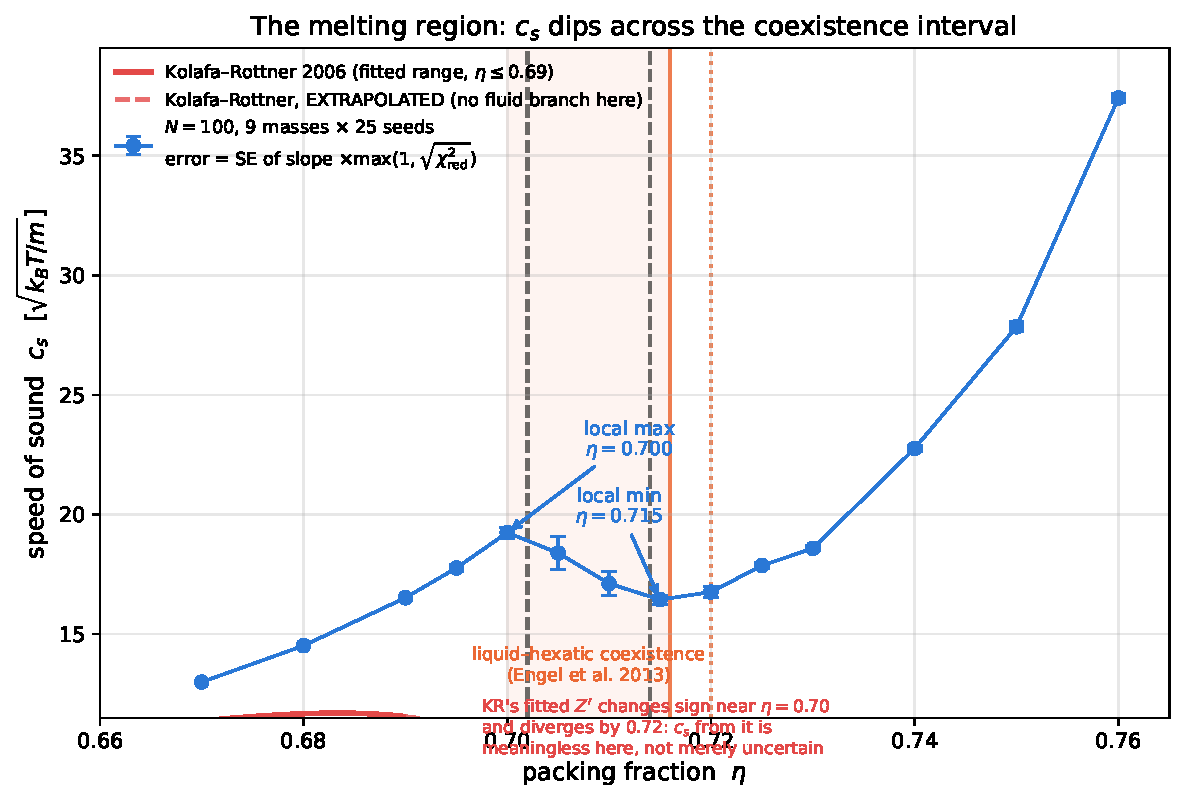
\includegraphics[width=\linewidth]{261002_p1_melting_region.pdf}
\caption{The melting region. Vertical lines are Engel \emph{et al.}'s independently measured
landmarks~\cite{engel2013}: the Mayer--Wood loop extrema at $\eta \approx 0.702$ and $0.714$, the
end of liquid--hexatic coexistence at $0.716$, and the hexatic--solid crossover at $0.720$. Our
$c_s$ turns over inside the same interval. Kolafa--Rottner is solid inside its fitted range and
dashed beyond it, and is cut off at $\eta = 0.705$ deliberately: its fitted $Z'$ runs $48$ at
$\eta = 0.67$, $28$ at $0.69$, $-9$ at $0.700$ and $+3386$ at $0.720$, so a $c_s$ built from it
there is meaningless rather than merely uncertain. The negative $Z'$ already inside the stated
fitted range is also why KR's own $c_s$ turns over near $\eta = 0.683$.}
\label{fig:melting}
\end{figure}

A caution that applies to the whole window, ours and theirs alike: $c_s$ is built from $Z'$, and
$Z'$ is where every equation of state is weakest. This is a \textbf{qualitative} correspondence and
is claimed as nothing more. Engel \emph{et al.}
work at $N = 256^2$ to $1024^2$; at $N = 100$ the Mayer--Wood loop is smeared over a width
comparable to its own depth, the first-order character cannot be resolved, and their tabulated
pressure exists at one density rather than as a table across the range, so no quantitative
comparison is available. What the correspondence does establish is that the structure in our
$c_s(\eta)$ above $0.69$ is the melting transition rather than an estimator artefact.

\section{Outlook}
Two measurements remain. A size ladder at $N \approx 1000$ across the full density range would turn
\S\ref{sec:finitesize}'s two-point extrapolation into a curve; and a size series at $\eta = 0.65$
would test whether the offset continues to close where the compartment is only six disk diameters
wide. Both are cluster jobs. Above $\eta \approx 0.69$ the comparison is with
Engel \emph{et al.}~\cite{engel2013} rather than with a fluid equation of state
(\S\ref{sec:ordering}); turning the qualitative correspondence found there into a quantitative one
needs a global equation of state with hexatic and solid branches~\cite{liu2021} and a box large
enough to resolve the Mayer--Wood loop, neither of which is available at $N = 100$.

\section*{Reproducibility}
Every campaign directory carries the exact command and the estimator geometry line. The geometry
constant and the estimator share one definition, and the analysis refuses to run on data whose
recorded wall thickness disagrees with it.
% TODO-source: validation/tests_20260913.py (WALL_T, l_eff, assert_wall_thickness)

\begin{thebibliography}{9}
\bibitem{kolafa2006} J.~Kolafa and M.~Rottner, ``Simulation-based equation of state of the hard disk
fluid and prediction of higher-order virial coefficients,'' \emph{Mol.\ Phys.}, vol.~104, 2006.
\bibitem{engel2013} M.~Engel, J.~A.~Anderson, S.~C.~Glotzer, M.~Isobe, E.~P.~Bernard and
W.~Krauth, ``Hard-disk equation of state: first-order liquid--hexatic transition in two dimensions
with three simulation methods,'' \emph{Phys.\ Rev.\ E}, vol.~87, p.~042134, 2013.
\bibitem{roman2002} F.~L.~Rom\'an, J.~A.~White, A.~Gonz\'alez and S.~Velasco, ``The speed of sound
in a hard disk gas: A computer simulation,'' \emph{Am.\ J.\ Phys.}, vol.~70, no.~8, pp.~847--851,
2002.
\bibitem{liu2021} H.~Liu, ``Global equation of state and phase transitions of the hard disc
systems,'' \emph{Mol.\ Phys.}, vol.~119, no.~10, 2021.
\end{thebibliography}

% ---------------------------------------------------------------------------------------------
% FIGURES: all four of the previously-missing figures were made on 2026-10-01 from existing CSVs
% and traces (no runs) by validation/paper1_figures_20261001.py, and are now in the text:
%   fig:slowmode, fig:floor (section \ref{sec:estimator}); fig:ladderline, fig:ladderres (section
%   \ref{sec:ladder}). Sources: 260914_A1v2_kmin_sensitivity{,_extended,_X2p5}.csv;
%   260915_A1v2_damping_cells.json; A1v2_20260914/eta_0p112200/m_*/ traces.
% NOTE the worked ladder line is at eta = 0.1122, NOT 0.10: the A1 v2 sweep has no 0.10 leaf, and
%   0.1122 is the density at which all nine masses were run.
% ---------------------------------------------------------------------------------------------

\end{document}
